%\documentclass{article}
\documentclass{article}
\usepackage{tikz}
\usepackage{tikz-dependency}
\usepackage{multirow}
\usepackage{caption} 
\captionsetup[table]{skip=10pt}
\usepackage{array}
\newcolumntype{C}[1]{>{\centering\let\newline\\\arraybackslash\hspace{0pt}}m{#1}}
\usepackage[T1]{fontenc}




\begin{document}

\begin{table}
  [ht] 
   \begin{tabular}{ c  | c | l  r } \hline 
      catena &  type & \hspace{1cm}HI & HF \hspace{1cm} \\
       \hline \multirow{2}{*}{parallel} & adverbs & \parbox[c]{14em}{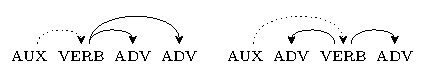
\includegraphics[width=5cm, height=1.5cm]{adverbs/ADV_ADV_V_HI.pdf}} &\parbox[c]{14em}{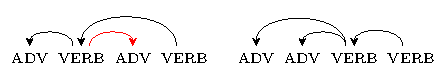
\includegraphics[width=5cm, height=1.5cm]{adverbs/ADV_ADV_V_HF.pdf}} \\
    & adjectives & \parbox[c]{14em}{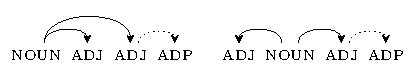
\includegraphics[width=5cm, height=1.5cm]{adjectives/ADJ_ADJ_N_HI.pdf}} &\parbox[c]{14em}{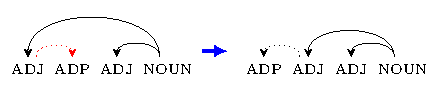
\includegraphics[width=5cm, height=1.5cm]{adjectives/ADJ_ADJ_N_HF.pdf}} \\
   \hline
 \multirow{4}{*}{hierarchical} & relative clause & \parbox[c]{14em}{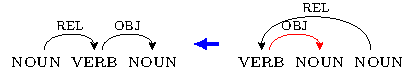
\includegraphics[width=5cm, height=1.5cm]{relative/REL_HI.pdf}} &\parbox[c]{14em}{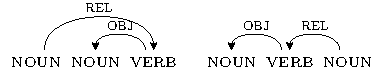
\includegraphics[width=5cm, height=1.5cm]{relative/REL_HF.pdf}} \\
 & complement clause & \parbox[c]{14em}{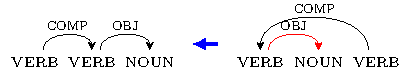
\includegraphics[width=5cm, height=1.5cm]{complement/COMP_HI.pdf}} &\parbox[c]{14em}{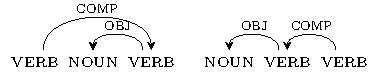
\includegraphics[width=5cm, height=1.5cm]{complement/COMP_HF.pdf}} \\
  & genitive & \parbox[c]{14em}{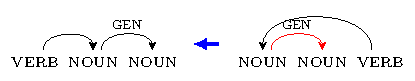
\includegraphics[width=5cm, height=1.5cm]{genitive/Gen_HI.pdf}} &\parbox[c]{14em}{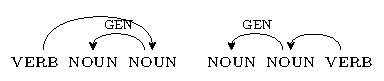
\includegraphics[width=5cm, height=1.5cm]{genitive/Gen_HF.pdf}} \\
    & adjective/adverb & \parbox[c]{14em}{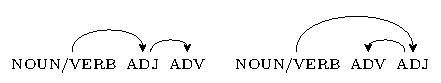
\includegraphics[width=5cm, height=1.5cm]{adjective_adverbs/ADJ_ADV_HI.pdf}} &\parbox[c]{14em}{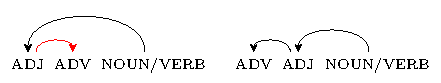
\includegraphics[width=5cm, height=1.5cm]{adjective_adverbs/ADJ_ADV_HF.pdf}} \\
    \hline
  \end{tabular}
\end{table}

\end{document}